% Figures
\afterpage{
     \begin{figure}[t!]
         \centering
         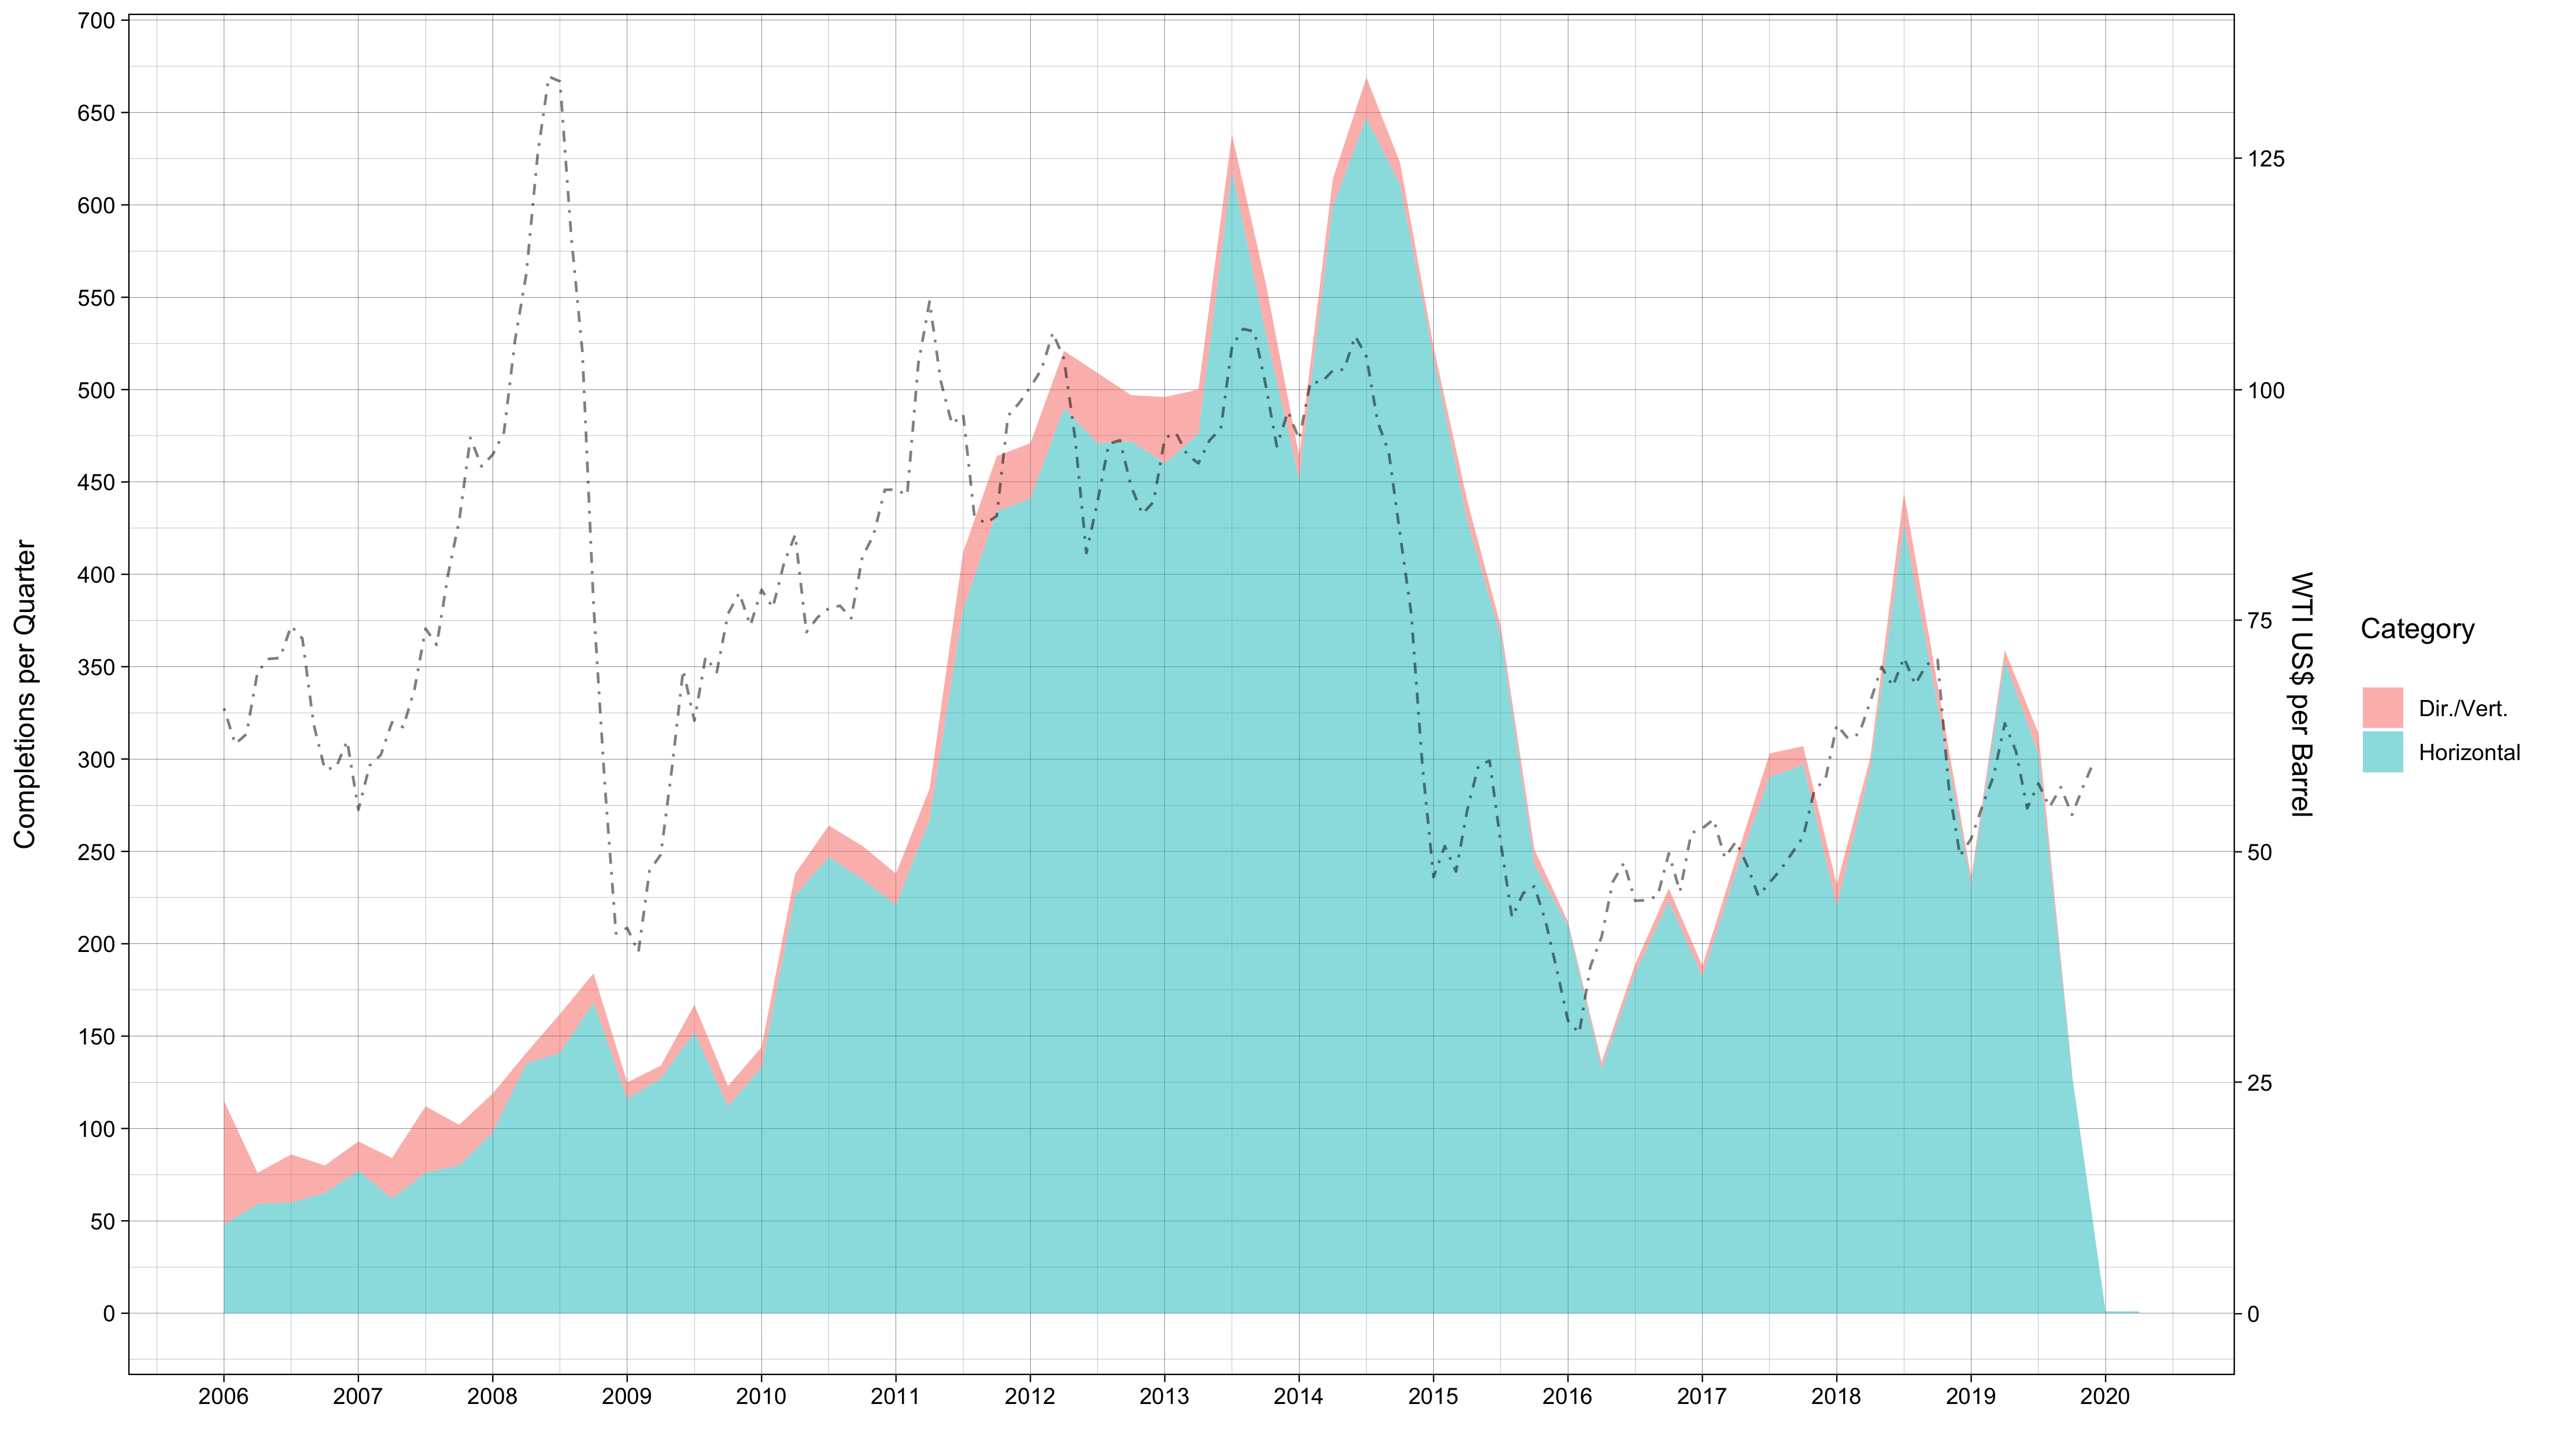
\includegraphics[scale = 0.11]{04_Chapter-3/00A_Figures/Completion-over-Time.png}
         \caption{Time Series of the Number of Drilling in North Dakota}
         \subcaption*{
             \textit{Note}: 
             This figure shows the time series of the number of well completions in North Dakota. Horizontal wells have been strictly dominant in that area. The dot-dashed line in the figure is the monthly per-barrel spot prices for West Texas Intermediate at Cushing, Oklahoma. The figure convincingly suggests that spot prices positively correlate with horizontal drilling in North Dakota. 
         }
         \label{Figure:Time-Series-of-the-Number-of-Drilling-in-North-Dakota}
     \end{figure}
 }
 \clearpage

\begin{landscape}
%\afterpage{
    \begin{figure}[t!]
        \centering
        \includegraphics[scale = 0.095]{04_Chapter-3/00A_Figures/Spatial-Distribution_Geological-Characteristics_Thermal-Maturity.png}
        \caption{Spatial Distributions of Geological Characteristics}
        \subcaption*{
            \textit{Note}: 
            This figure depicts the spatial distributions of three geological features---thickness, thermal maturity, and total organic contents---, which are available from the NDGS' geological survey data. In this figure, each dot indicates an individual well. 
        }
        \label{Figure:Spatial-Distributions-of-Geological-Characteristics}
    \end{figure}
% }
\end{landscape}
% \clearpage

\begin{landscape}
%\afterpage{
    \begin{figure}[t!]
        \centering
        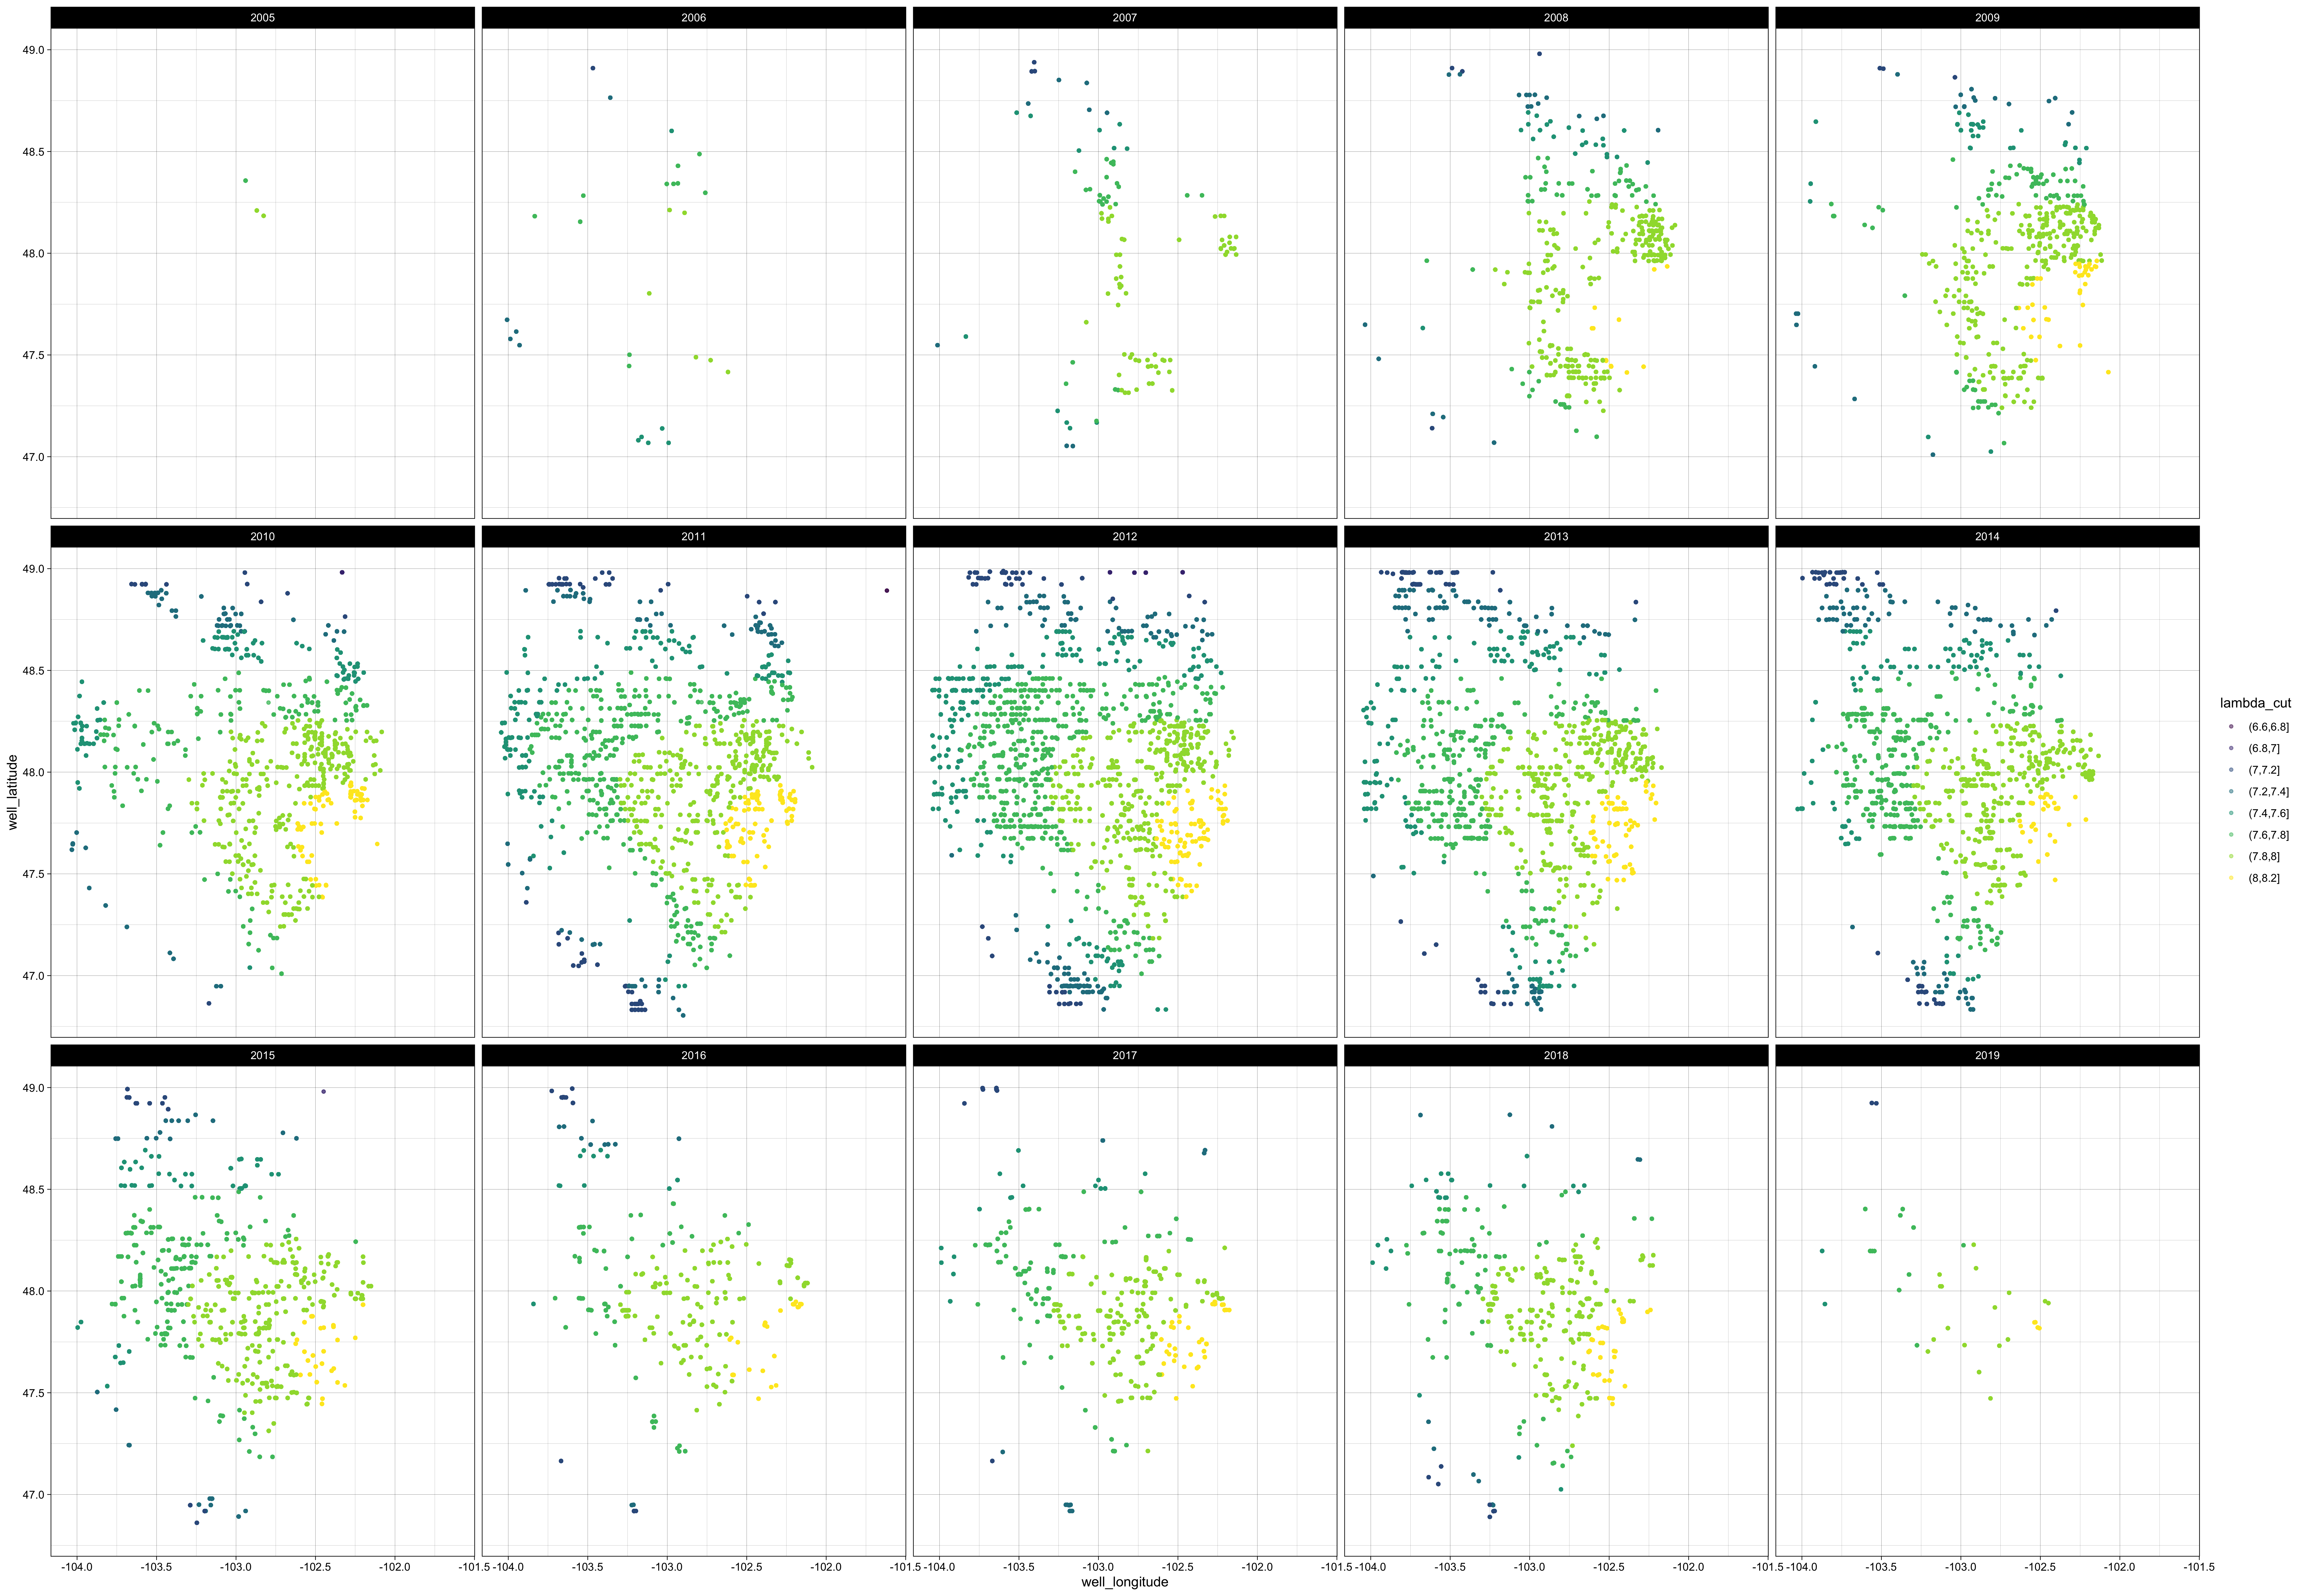
\includegraphics[scale = 0.075]{04_Chapter-3/00A_Figures/Robinson-Estimator_Productivity-across-Locations_Discrete.png}
        \caption{Spatial Distribution of the Estimated Geological Characteristic by Year}
        \subcaption*{
            \textit{Note}: 
            This figure illustrates the estimated geologic feature for each horizontal well by year. It is apparent that the share of drilling of horizontal wells with (relatively) small estimates decreased significantly starting in 2014, corresponding to the beginning of the oil price crash.
        }
        \label{Figure:Spatial-Distribution-of-the-Estimated-Geological-Characteristic-by-Year}
    \end{figure}
%}
\end{landscape}
\clearpage

\afterpage{
    \begin{figure}[t!]
        \centering
        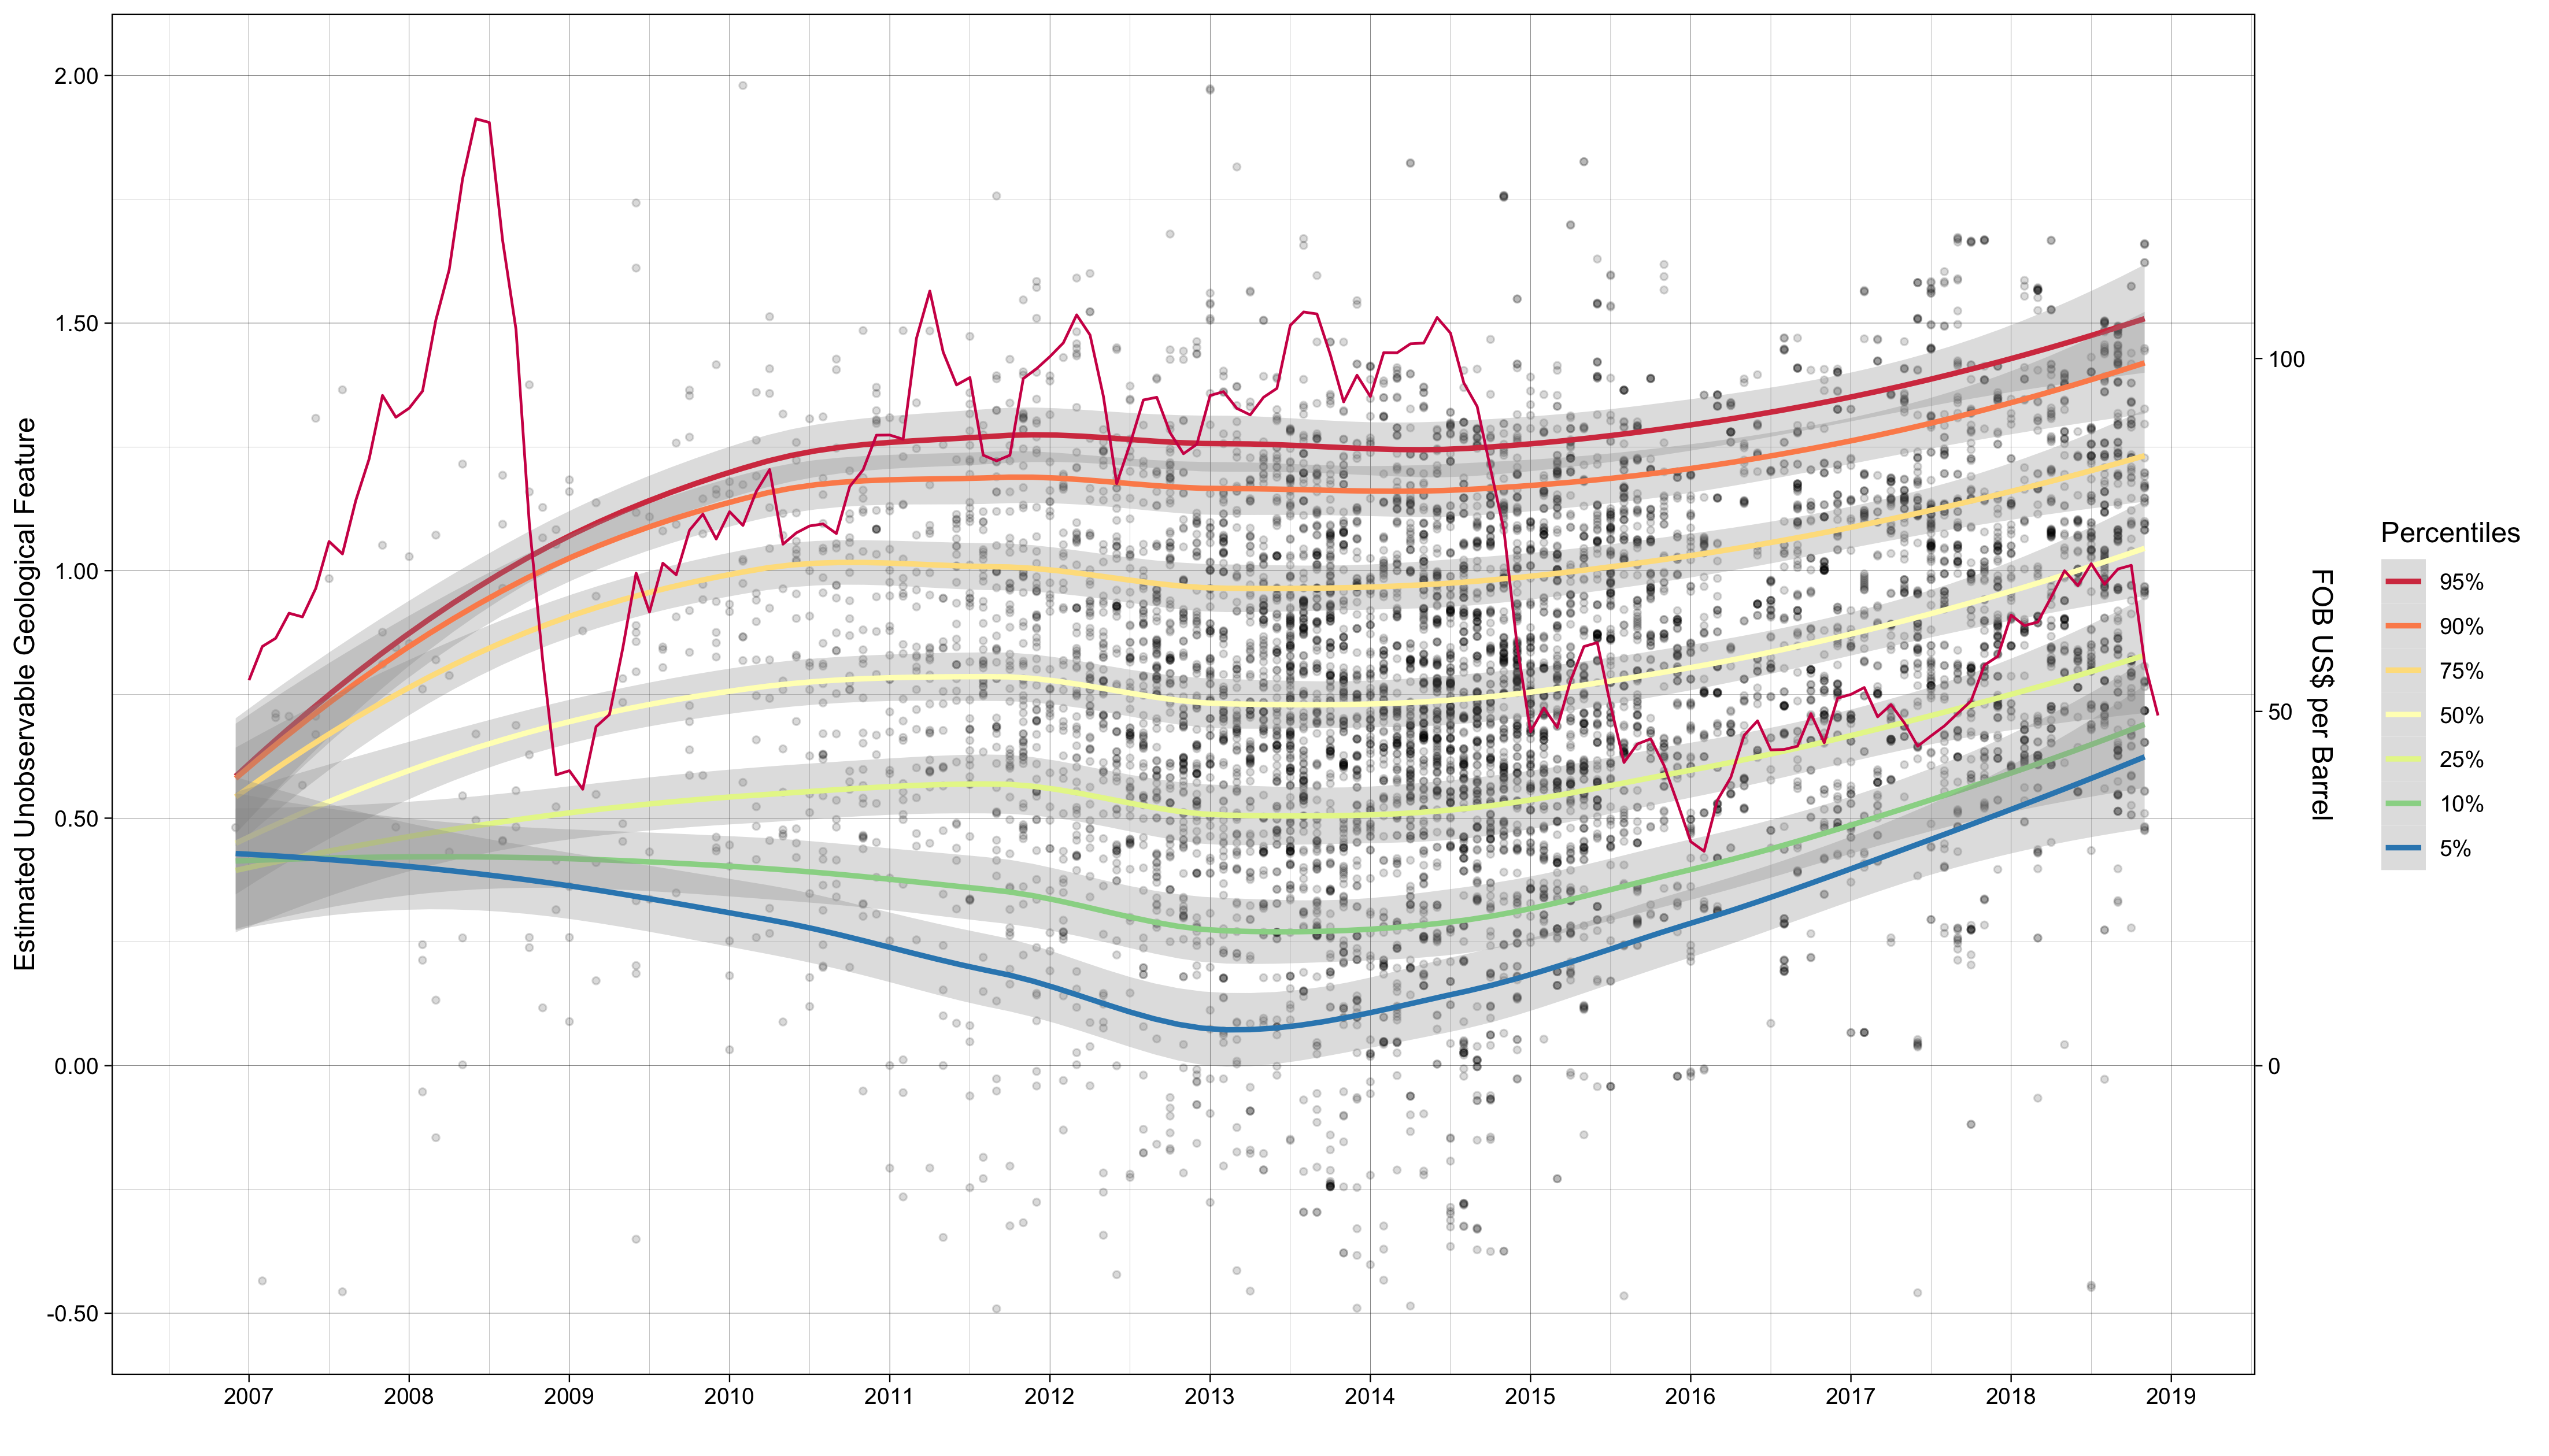
\includegraphics[scale = 0.1]{04_Chapter-3/00A_Figures/Cross-Sectional-Approach_Estimates-from-Robinson-Estimator_Time-Trend_Unobservable-Geology.png}
        \caption{Simultaneous Drilling of Horizontal Wells with Heterogeneous Geological Quality}
        \subcaption*{
            \textit{Note}: 
            This figure indicates the estimated geological feature for each horizontal well, depicted as a dot. Those dots definitely suggest the simultaneous drilling of horizontal wells with heterogeneous geological quality. In the figure, percentiles of the estimates, with the 95\% confidence interval of each, are also presented. The dot-dashed line is the time series of the monthly per-barrel spot prices for West Texas Intermediate at Cushing, Oklahoma. Oil prices plunged significantly between 2014 and 2015 and rose gradually. The percentile lines skewed upward, especially lower ones, as of the second half of 2014. 
        }
        \label{Figure:Simultaneous-Drilling-of-Horizontal-Wells-with-Heterogeneous-Geological-Quality}
    \end{figure}
}
\clearpage

\afterpage{
    \begin{figure}[t!]
        \centering
        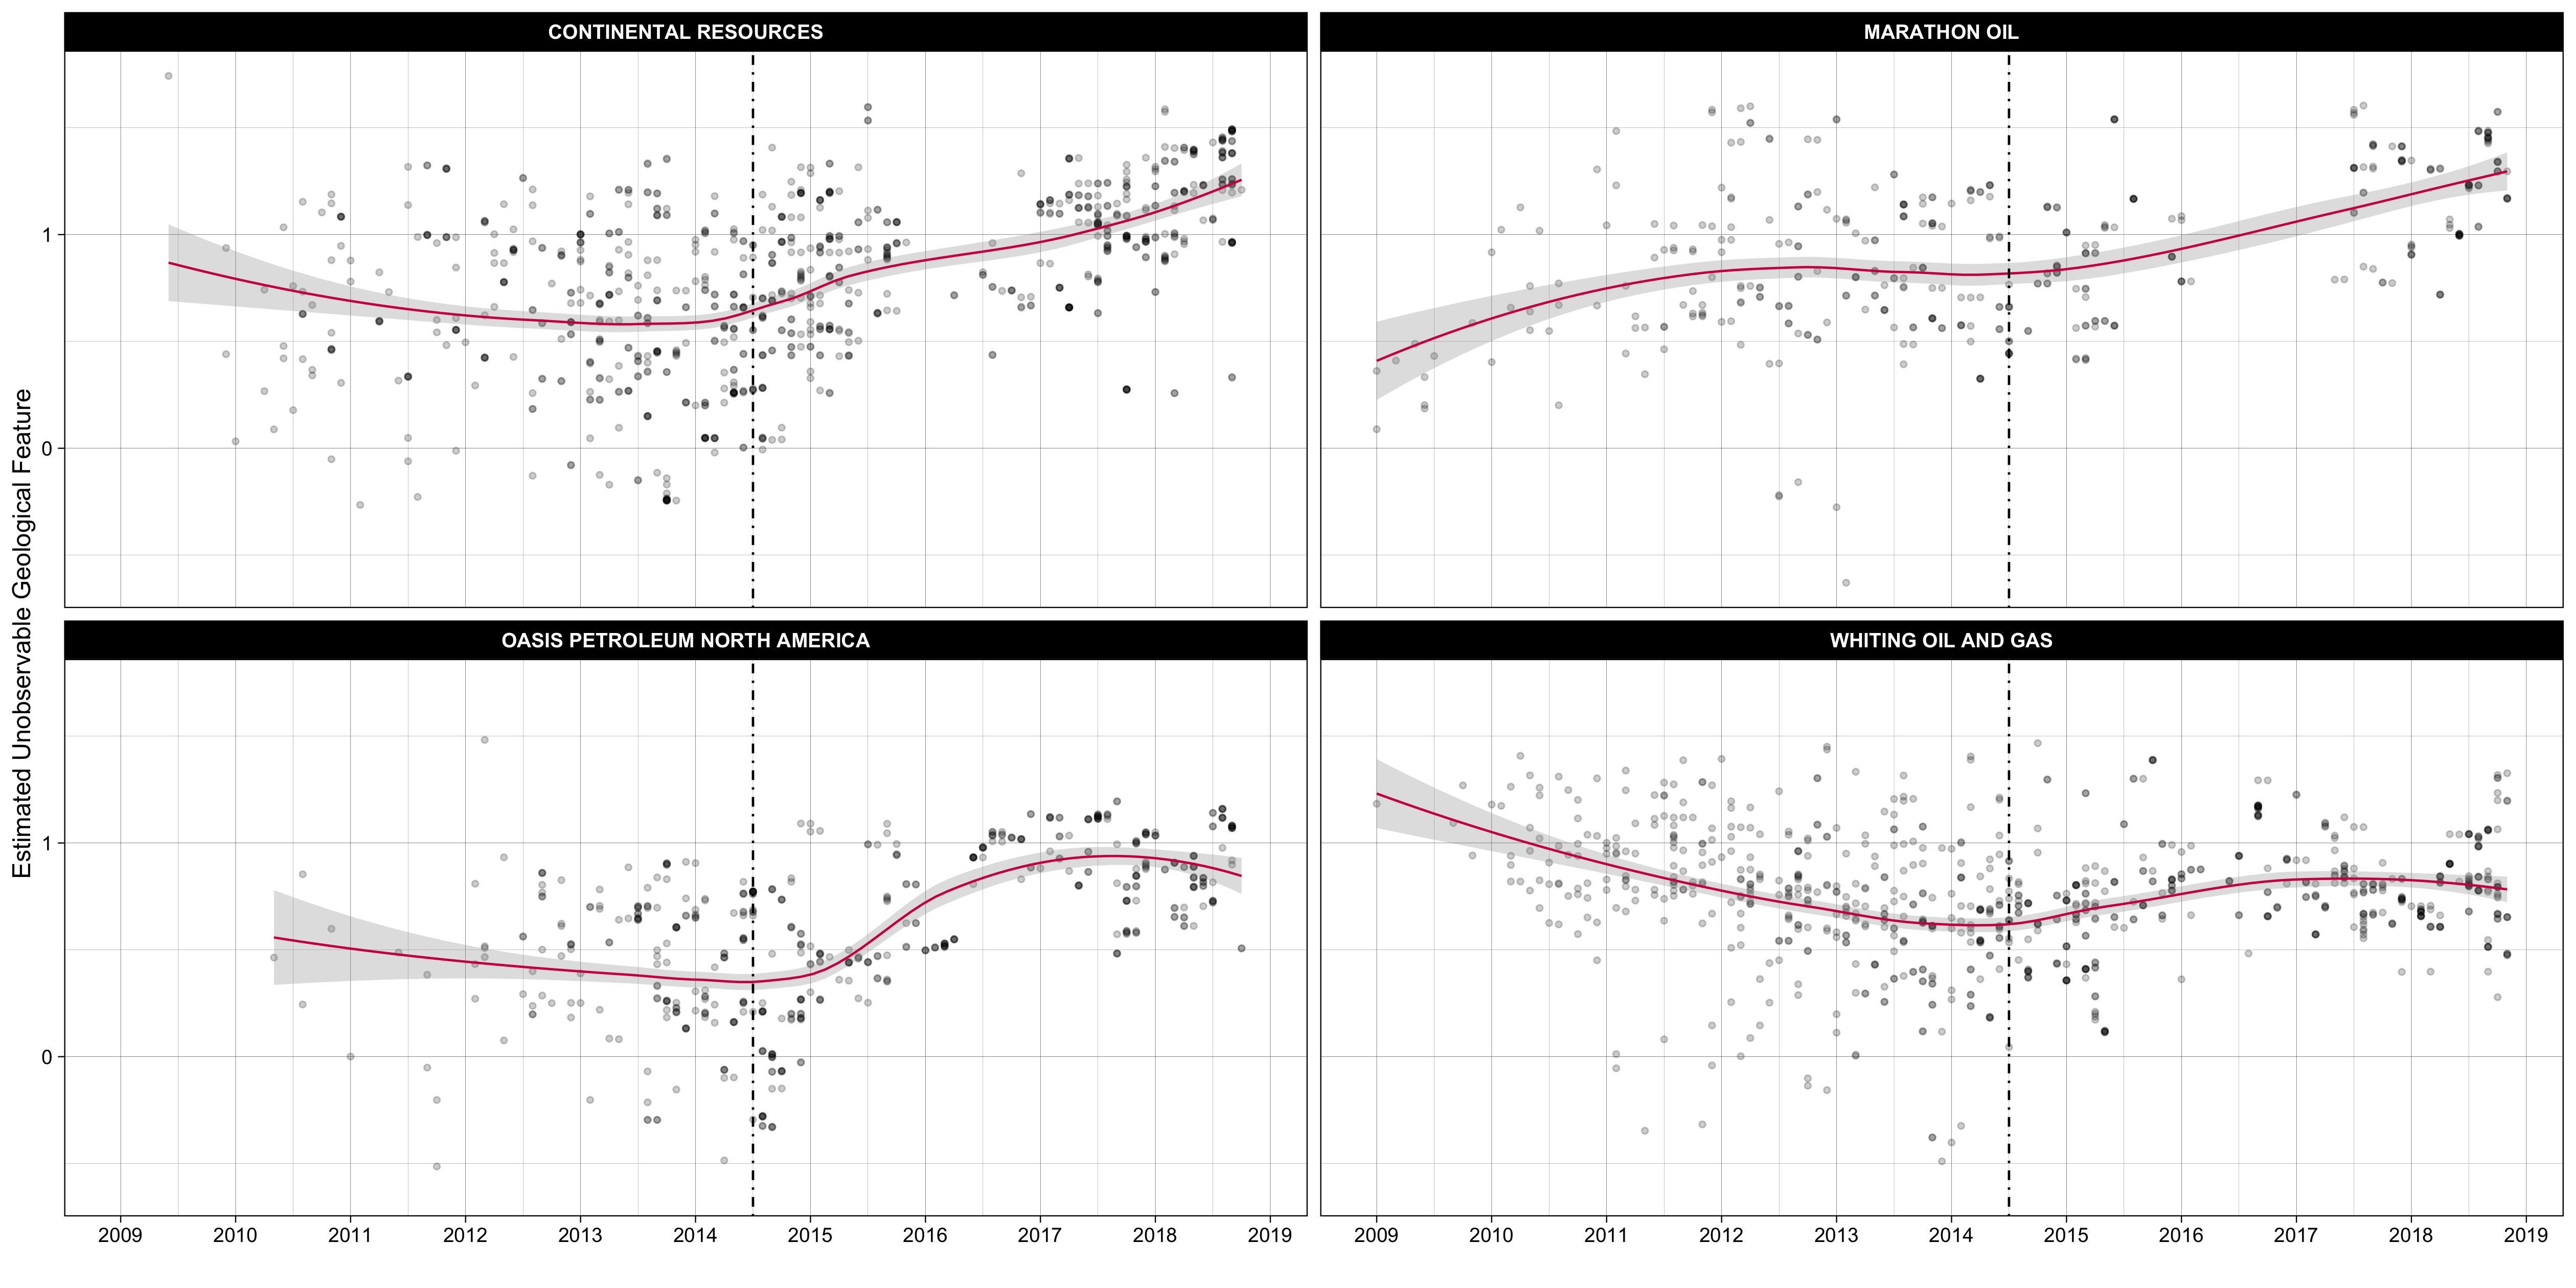
\includegraphics[scale = 0.095]{04_Chapter-3/00A_Figures/Estimates-from-Robinson-Estimator_By-Firm.png}
        \caption{High Sensitivity of Firm-Level Low-Quality Well Drilling to the Negative Price Shocks in 2014-15}
        \subcaption*{
            \textit{Note}: 
            This figure shows how each of the four firms' drilling activity changed over time. Each dot in the figure indicates an individual well's estimated geological feature. The red line, with the 95\% confidence interval, in each panel demonstrates the average quality of horizontal wells drilled in a month. As illustrated, the firms significantly reduced drilling low-quality well locations since mid-2014, corresponding to the beginning of the oil price plunge.
        }
        \label{Figure:High-Sensitivity-of-Firm-Level-Low-Quality-Well-Drilling}
    \end{figure}
}
\clearpage

\afterpage{
    \begin{figure}[t!]
        \centering
        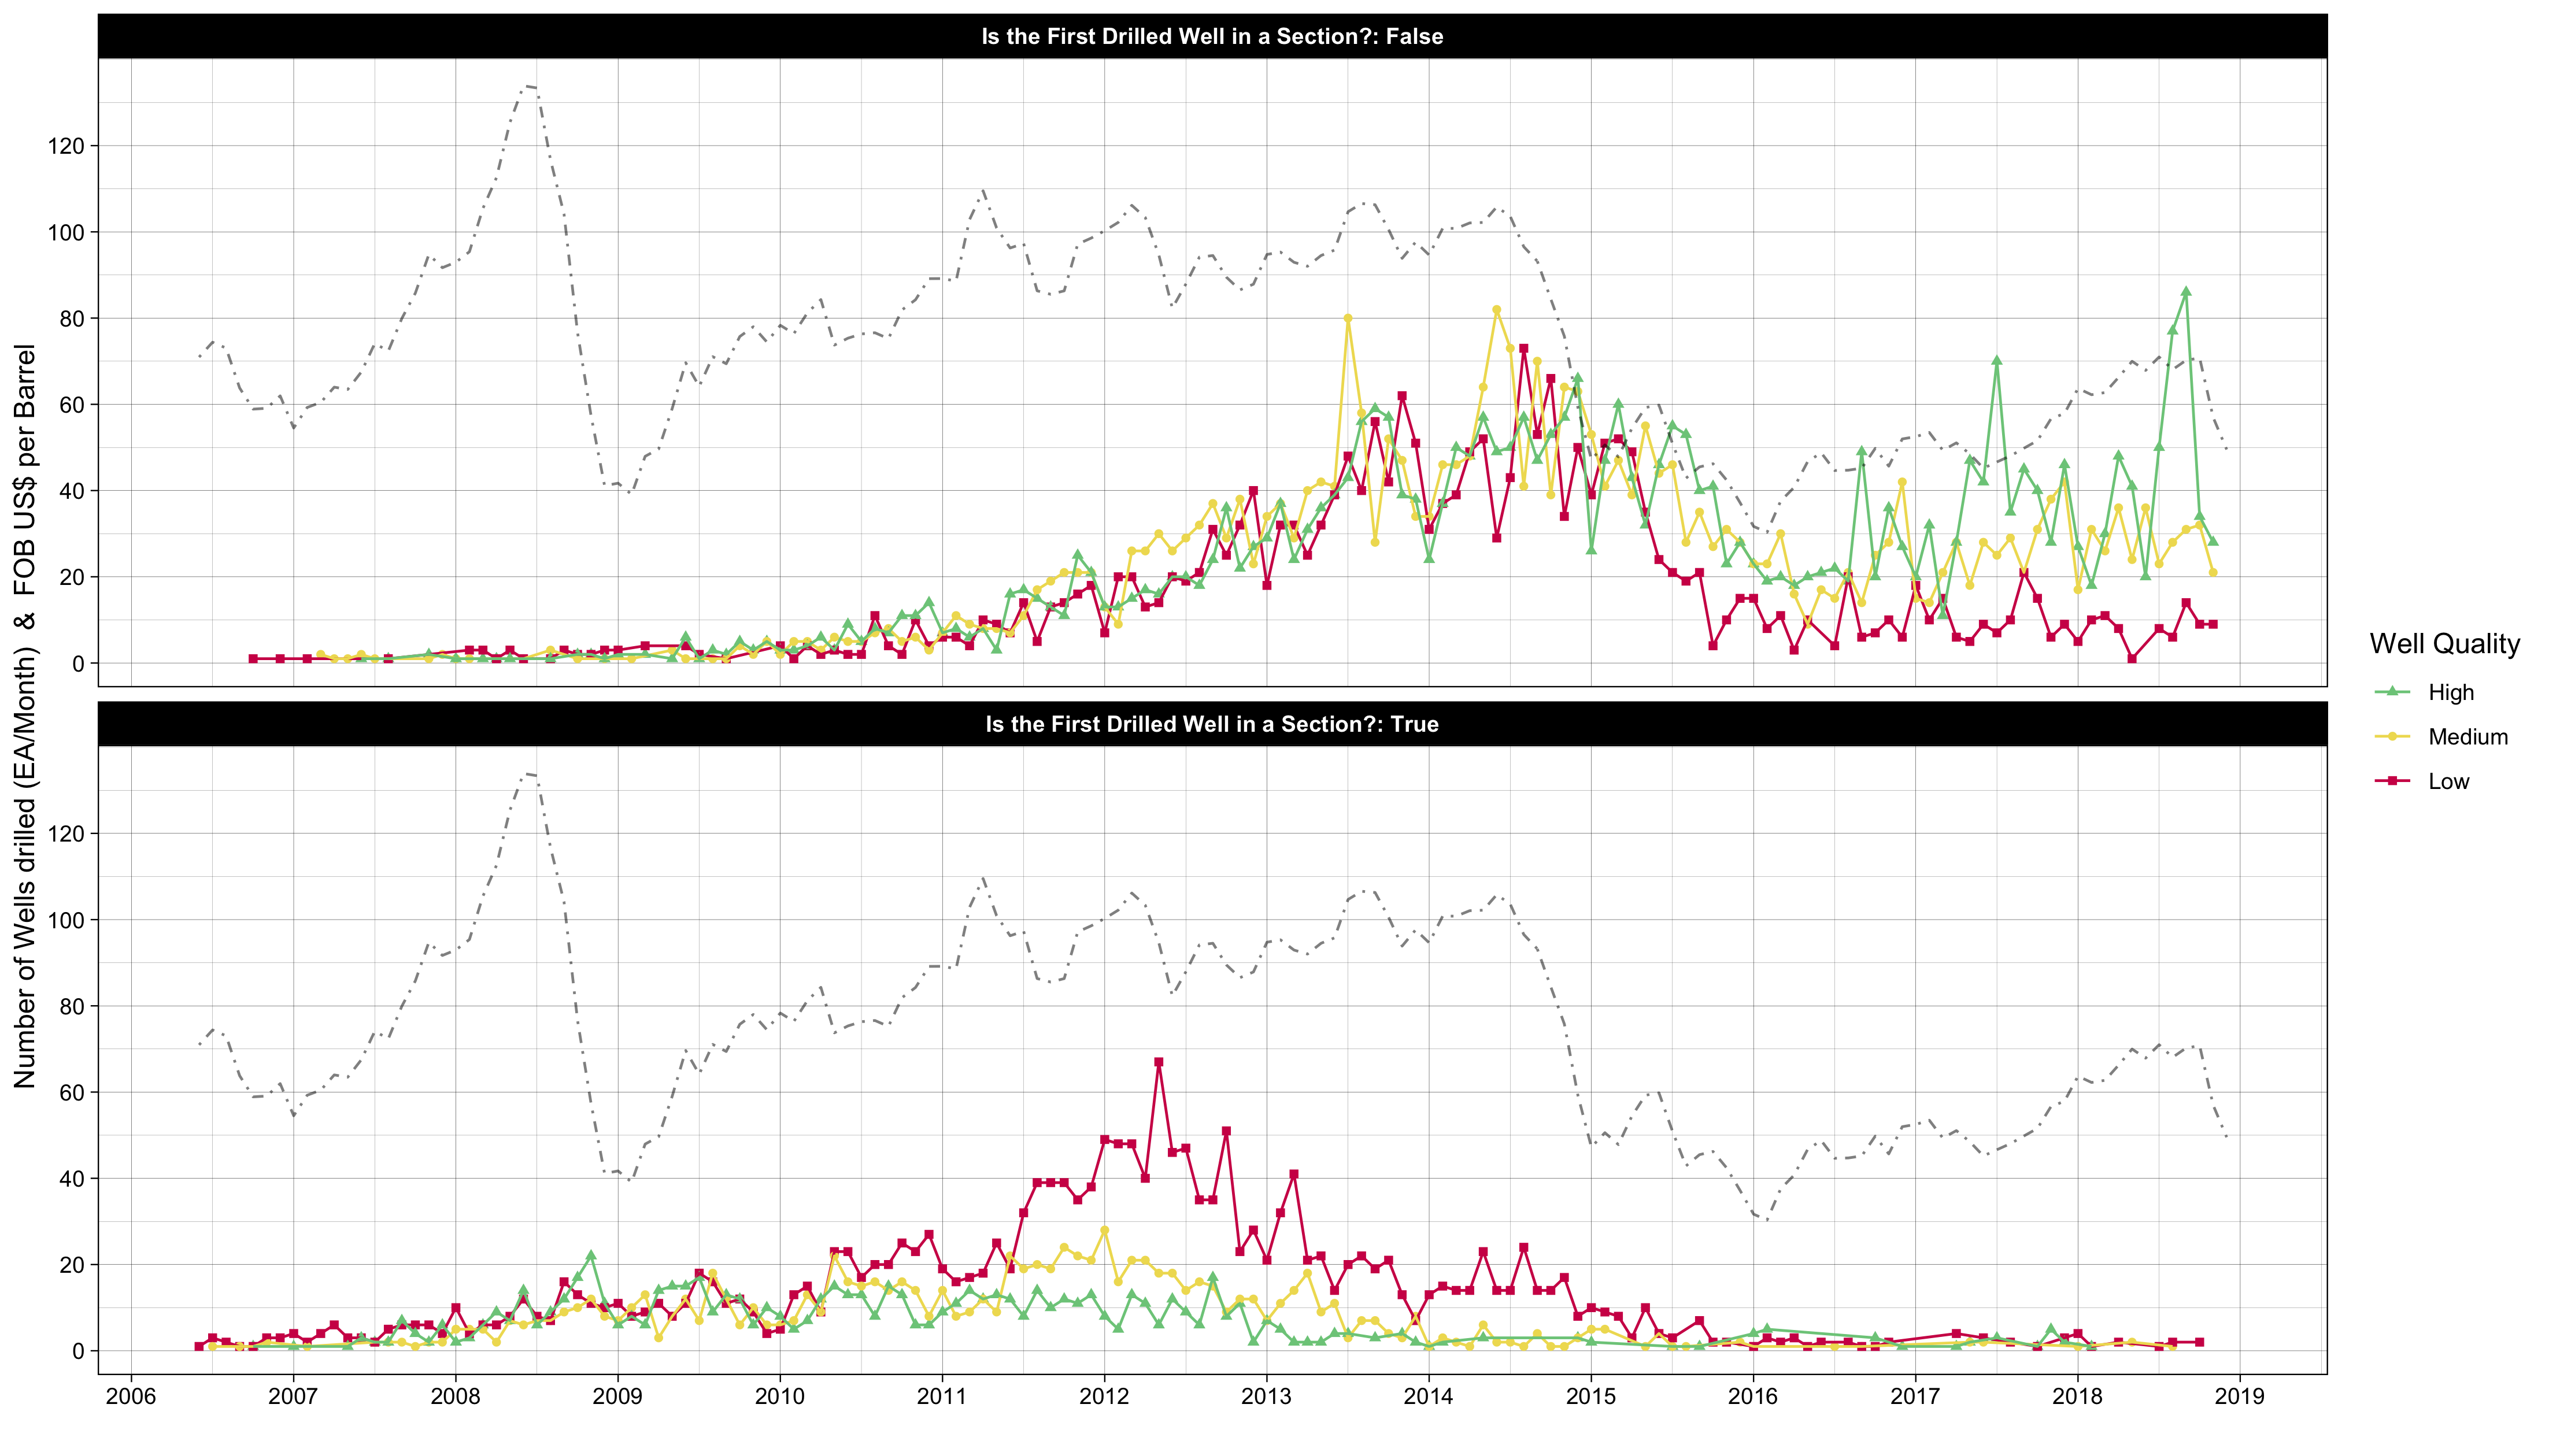
\includegraphics[scale = 0.11]{04_Chapter-3/00A_Figures/Drilling-over-Time_By-Well-Quality-and-Whether-First-Drilled.png}
        \caption{Held-by-Production vs. Non-Held-by-Production Horizontal Well Drilling}
        \subcaption*{
            \textit{Note}: 
            This figure depicts the drilling of horizontal wells classified into three quality levels. Drilling described in the upper panel is the first in each section, regarded as held-by-production drilling. There was only a limited number of held-by-production drilling between 2015 and 2019. The lower panel indicates all subsequent drilling in sections. The collapse in oil prices between mid-2014 and 2015 made post-held-by-production drilling decrease. Drilling of high-quality well sites was more responsive to the recovery of oil prices from 2016 to 2019. In each panel, the dot-dashed line is the time series of the monthly per-barrel spot prices for West Texas Intermediate at Cushing, Oklahoma.
        }
        \label{Figure:Held-by-Production-vs-Non-Held-by-Production-Horizontal-Well-Drilling}
    \end{figure}
}
\clearpage

\afterpage{
    \begin{figure}[t!]
        \centering
        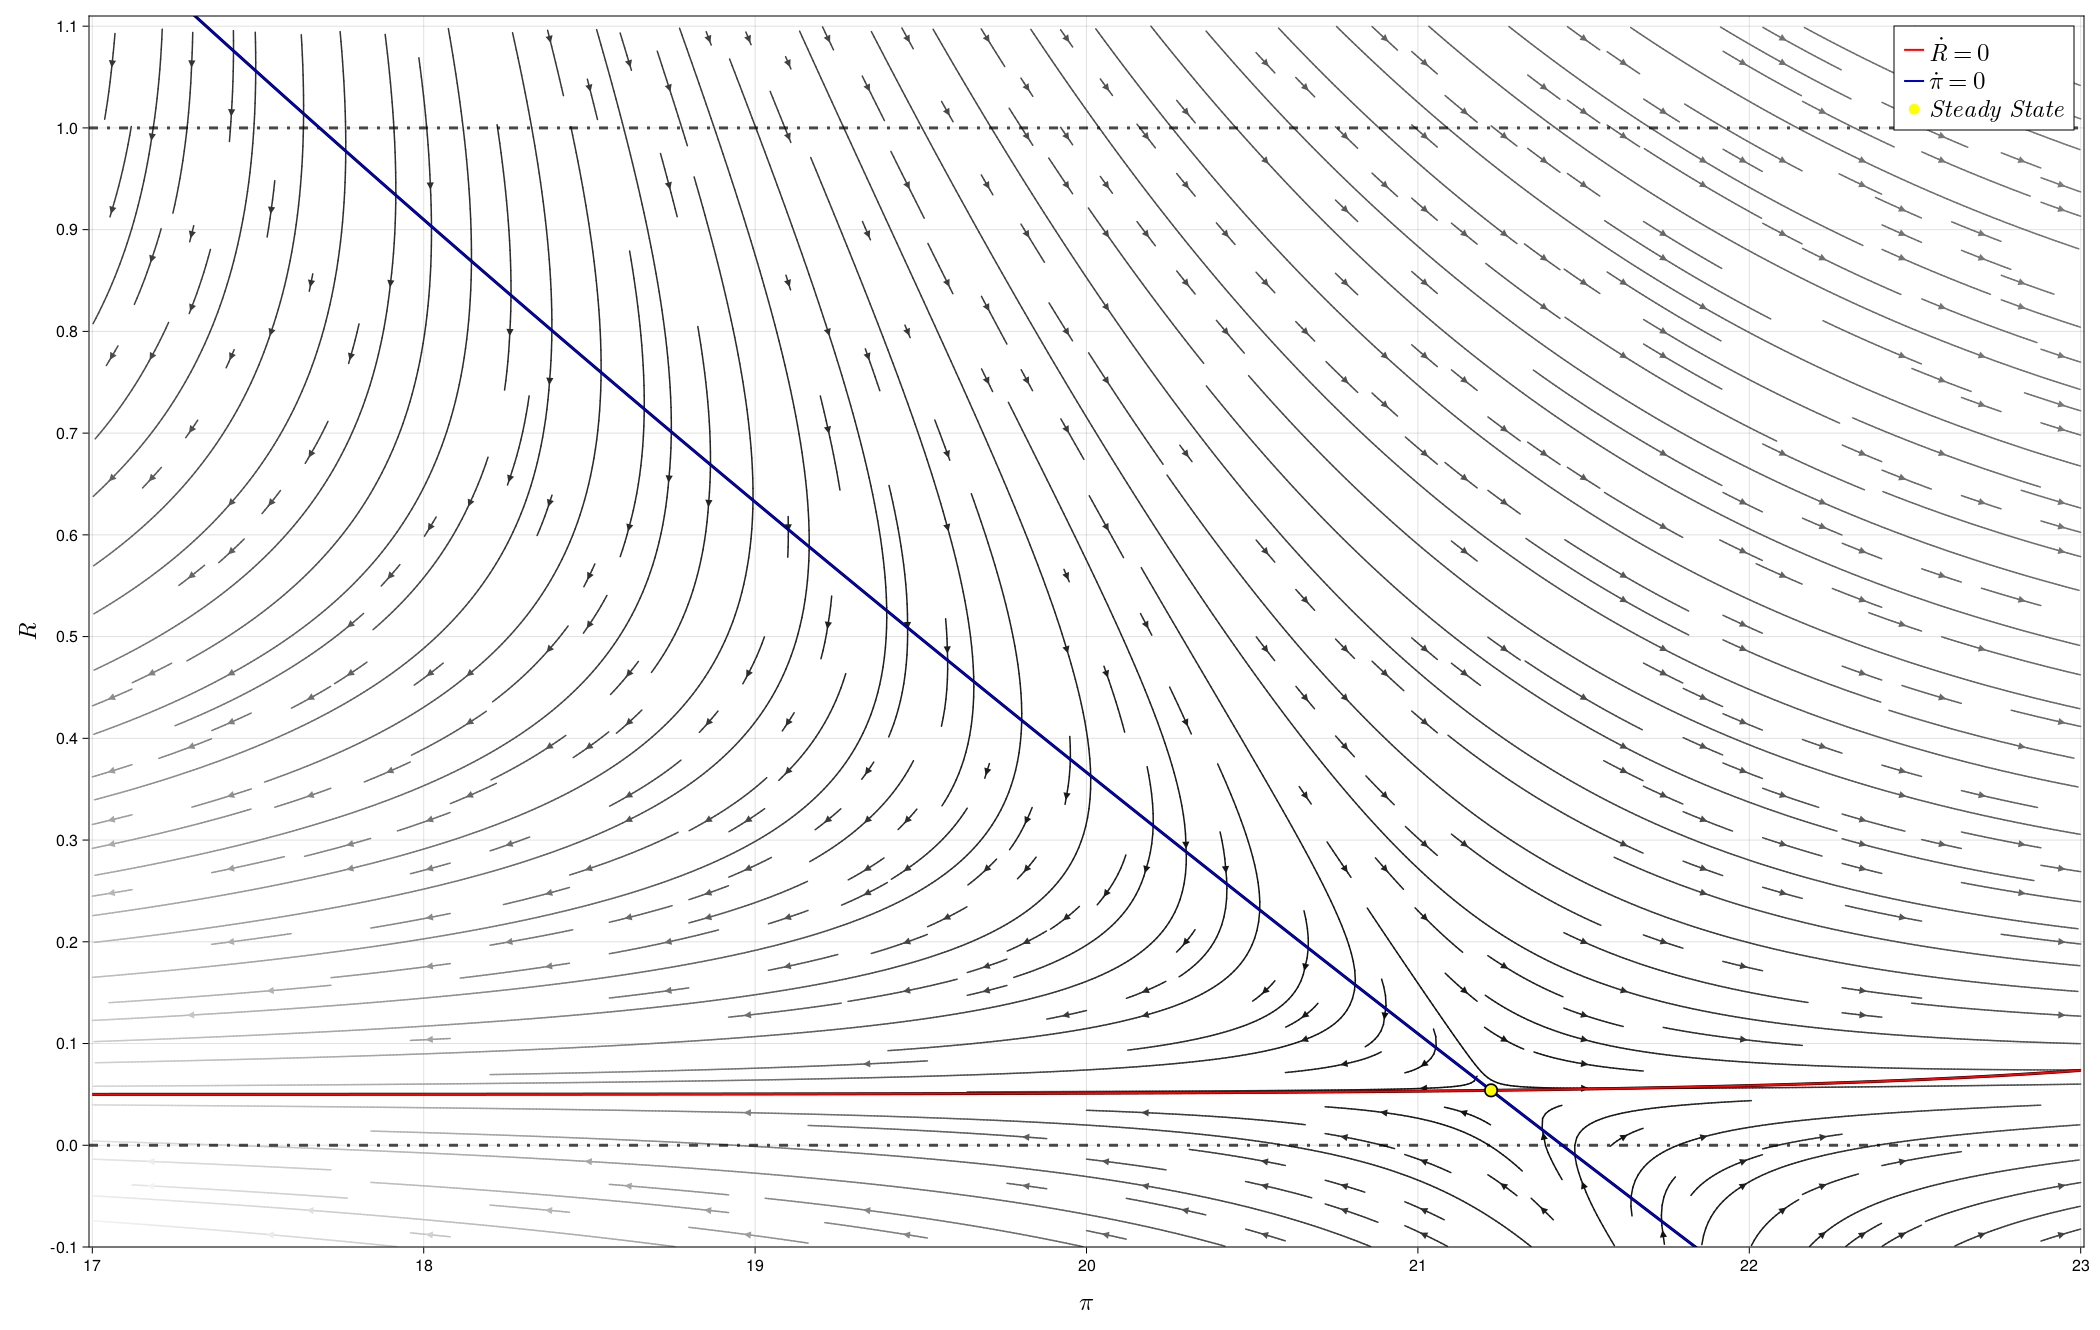
\includegraphics[scale = 0.20]{04_Chapter-3/00A_Figures/Figure_Equilibrium-Path_Exogenous-Price_Phase-Diagram_pi-by-R.png}
        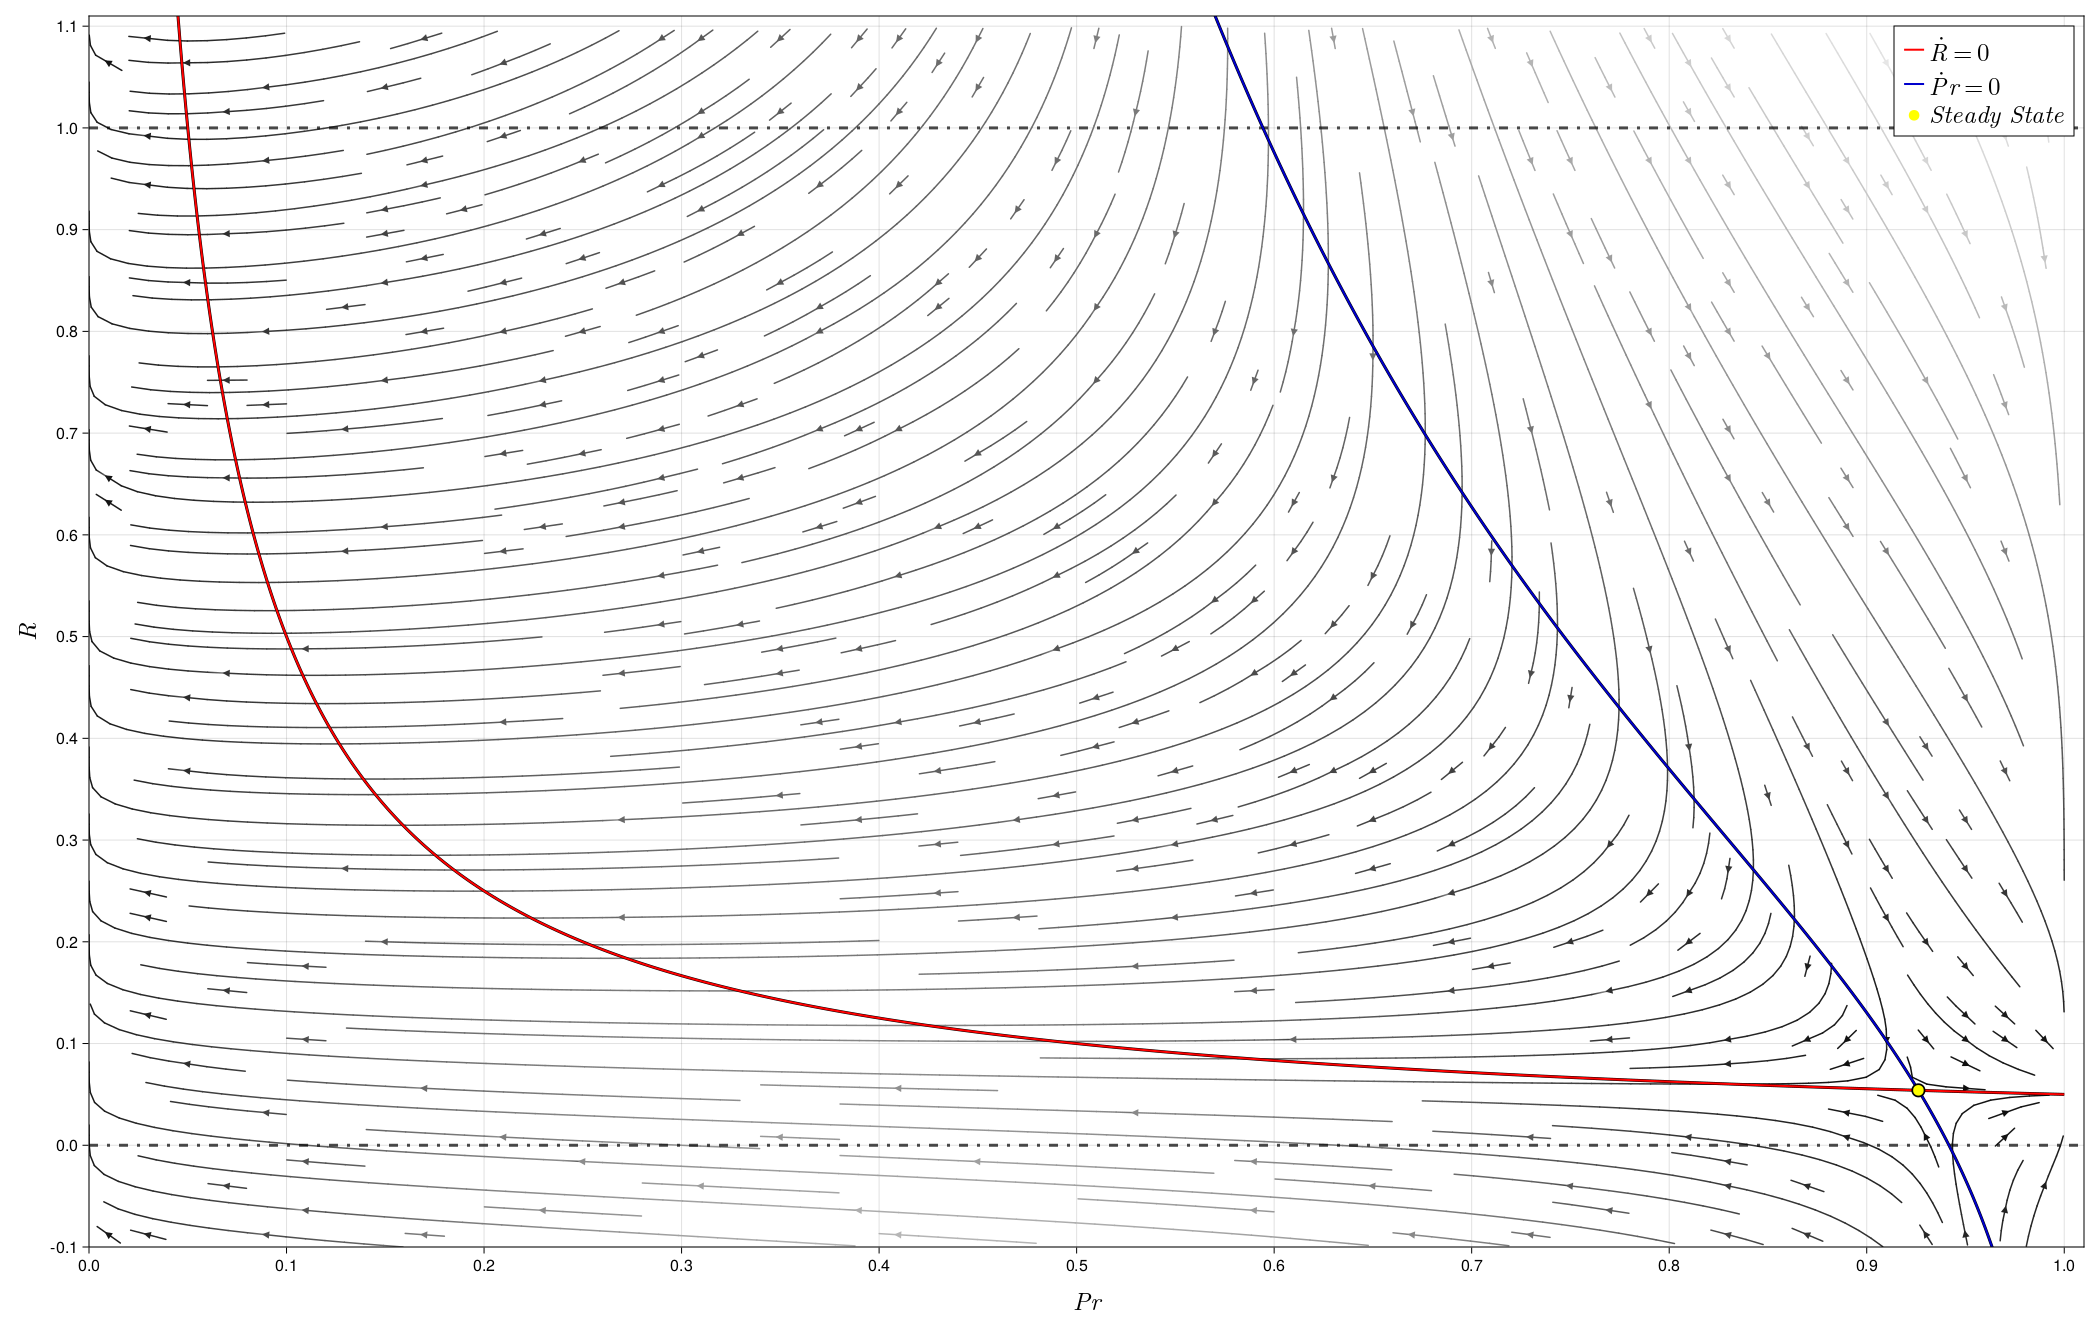
\includegraphics[scale = 0.20]{04_Chapter-3/00A_Figures/Figure_Equilibrium-Path_Exogenous-Price_Phase-Diagram_Pr-by-R.png}
        \caption{Phase Diagrams for the Social Planner's Problem}
        \subcaption*{
            \textit{Note}: 
            This figure shows two phase diagrams for the social planner's problem. The upper diagram illustrates that the steady state is exactly a saddle point. This figure assumes that a dispersion parameter of $\sigma = 1$, an interest rate of $r = 0.15$, initial reserves of $R_{0} = 1$, additional reserves of $E = 0.05$, and exogenously given constant oil prices of $\bar{p} = 50$. Also, a linear marginal cost function of $c'(D_{t}) = 1 + 5D_{t}$ is assumed.  
        }
        \label{Figure:Phase-Diagram_Saddle-Point}
    \end{figure}
}
\clearpage

\afterpage{
    \begin{figure}[t!]
        \centering
        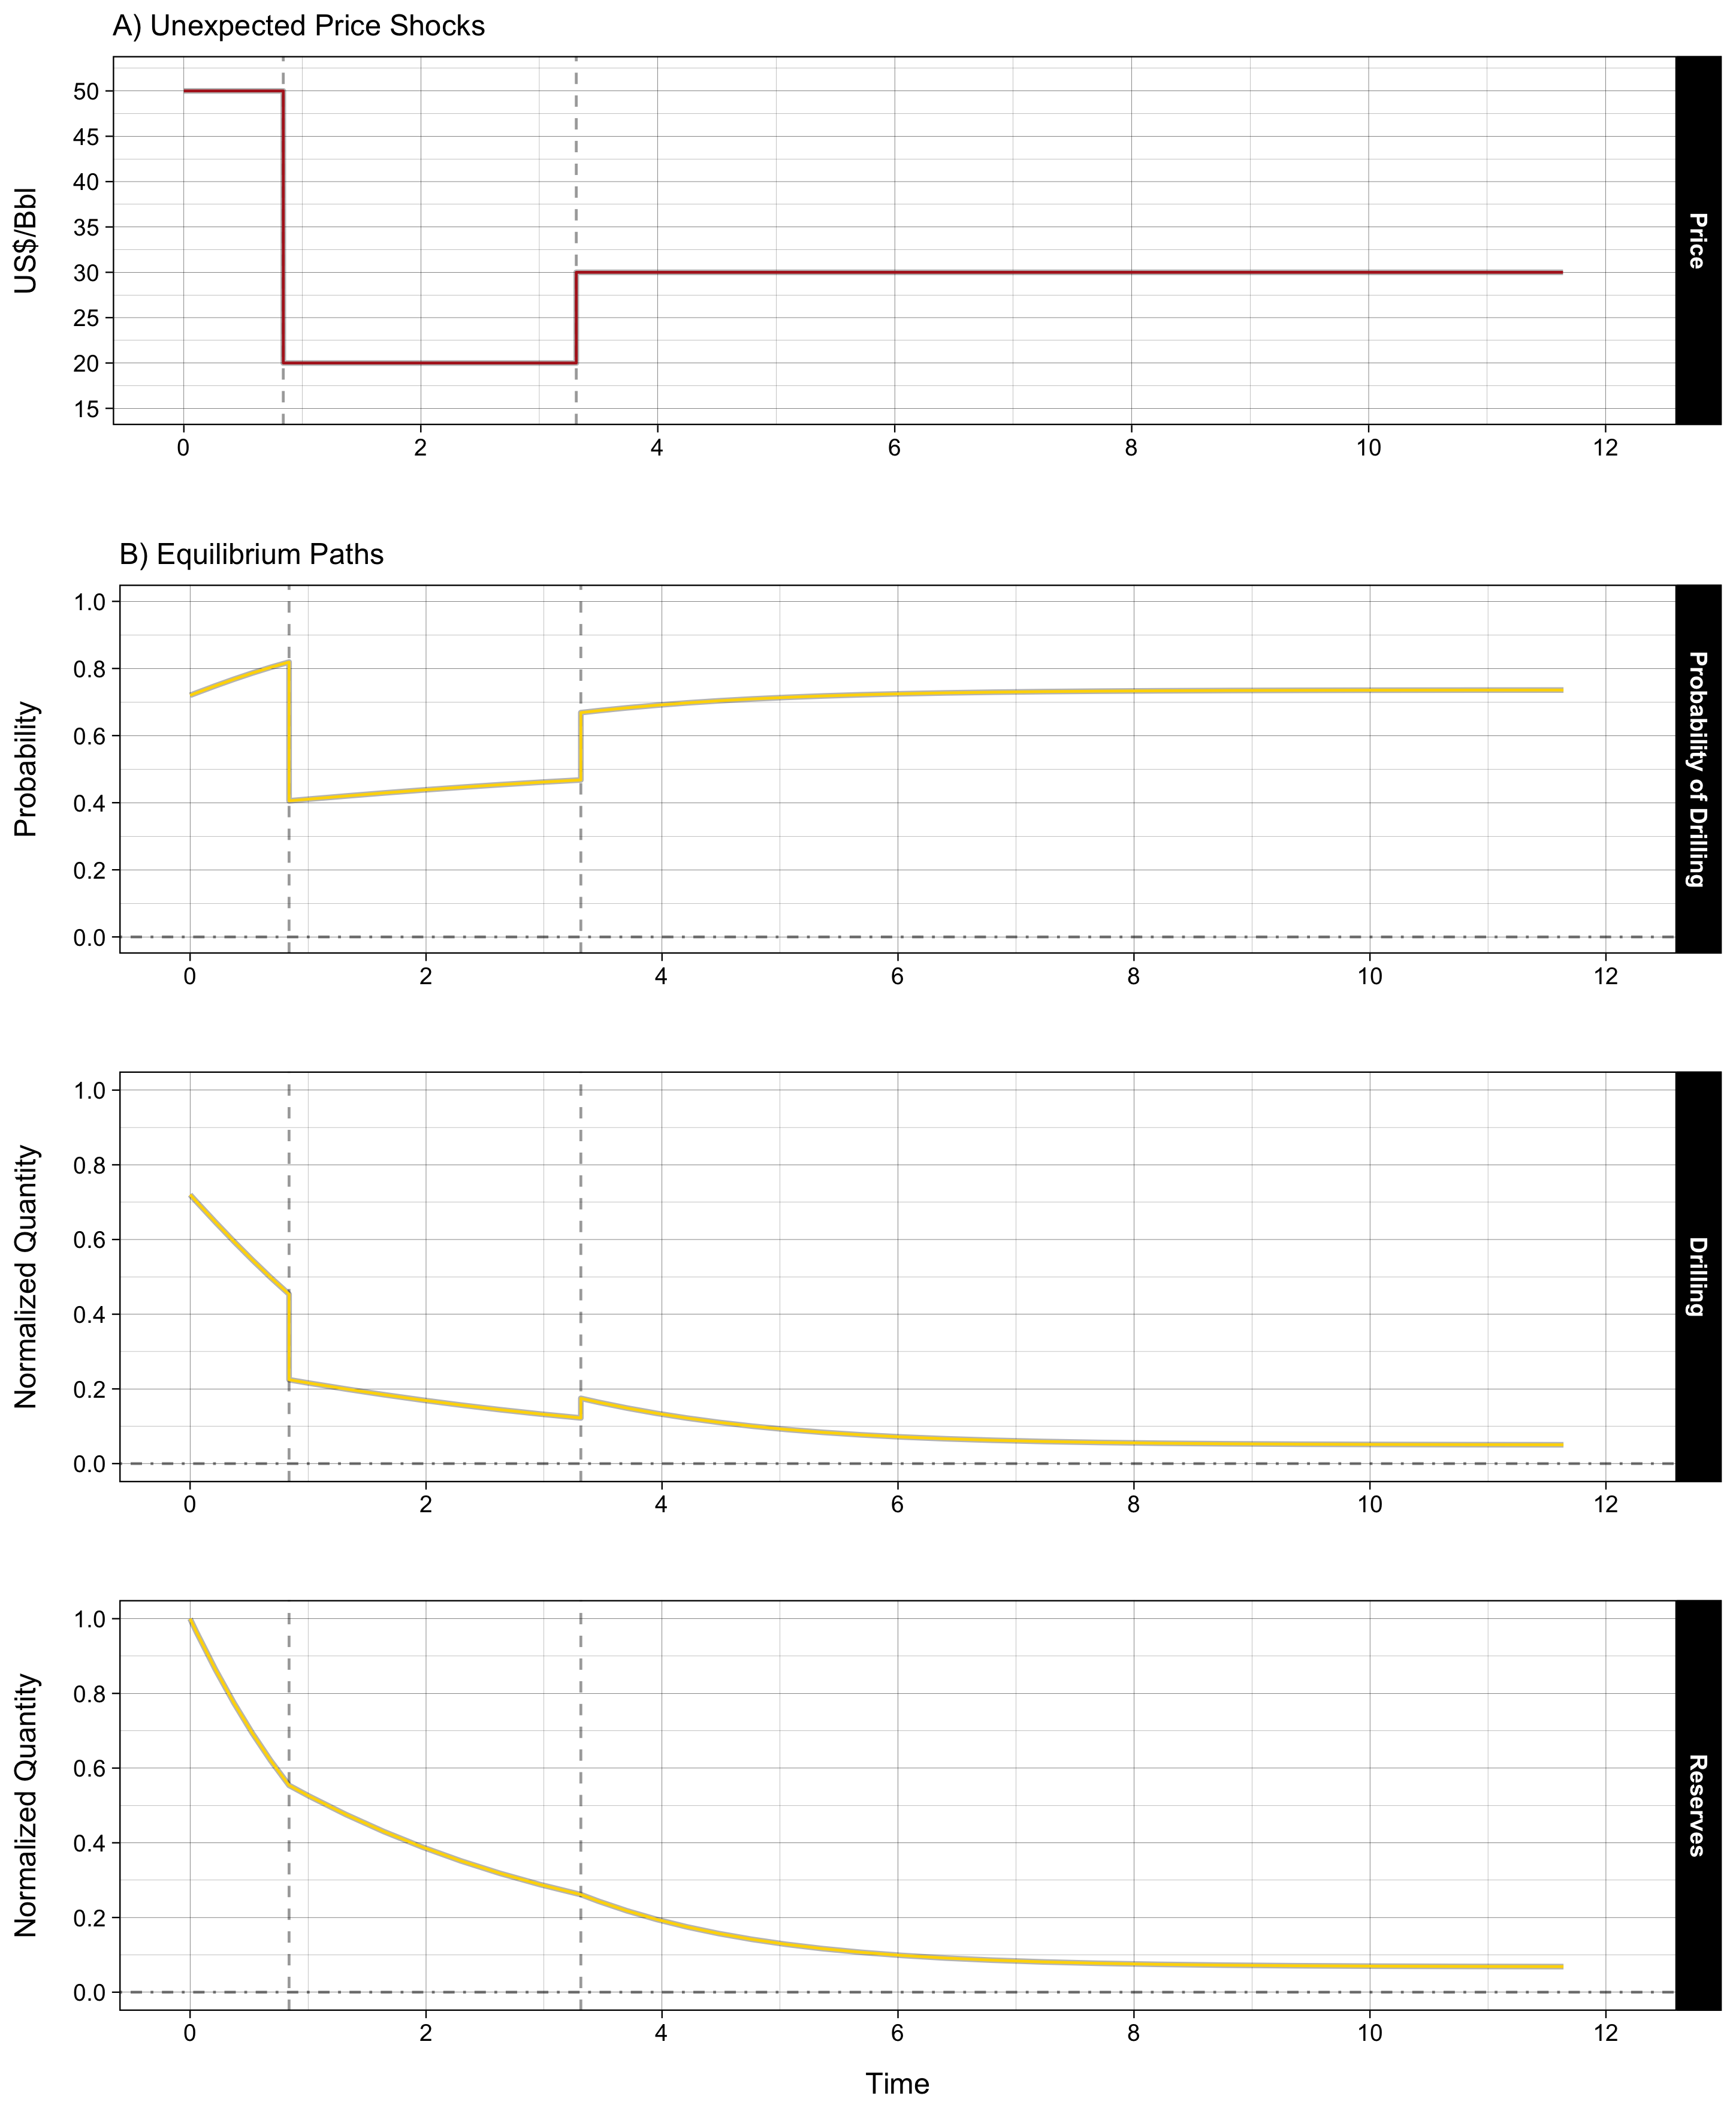
\includegraphics[scale = 0.15]{04_Chapter-3/00A_Figures/Figure_Equlibrium-Paths_Exogenous-Price.png}
        \caption{Equilibrium Paths under Unexpected Price Shocks}
        \subcaption*{
            \textit{Note}: 
            This figure shows the equilibrium paths for drilling probability, drilling, and undrilled reserves for exogenously given oil prices, including two unanticipated price shocks. This figure assumes the identical parameter values and the marginal cost function utilized to draw the phase diagrams in Figure \ref{Figure:Phase-Diagram_Saddle-Point}.
        }
        \label{Figure:Equilibrium-Paths-under-Unexpected-Price-Shocks}
    \end{figure}
}
\clearpage

\afterpage{
    \begin{figure}[t!]
        \centering
%        \includegraphics[scale = 0.1]{}
        \caption{Heterogeneous Impacts of Unexpected Price Shocks on Equilibrium Paths}
        \subcaption*{
            \textit{Note}: 
            (...)
        }
        \label{Figure:Heterogeneous-Impacts-of-Unexpected-Price-Shocks-on-Equilibrium-Paths}
    \end{figure}
}
\clearpage

\afterpage{
    \begin{figure}[t!]
        \centering
        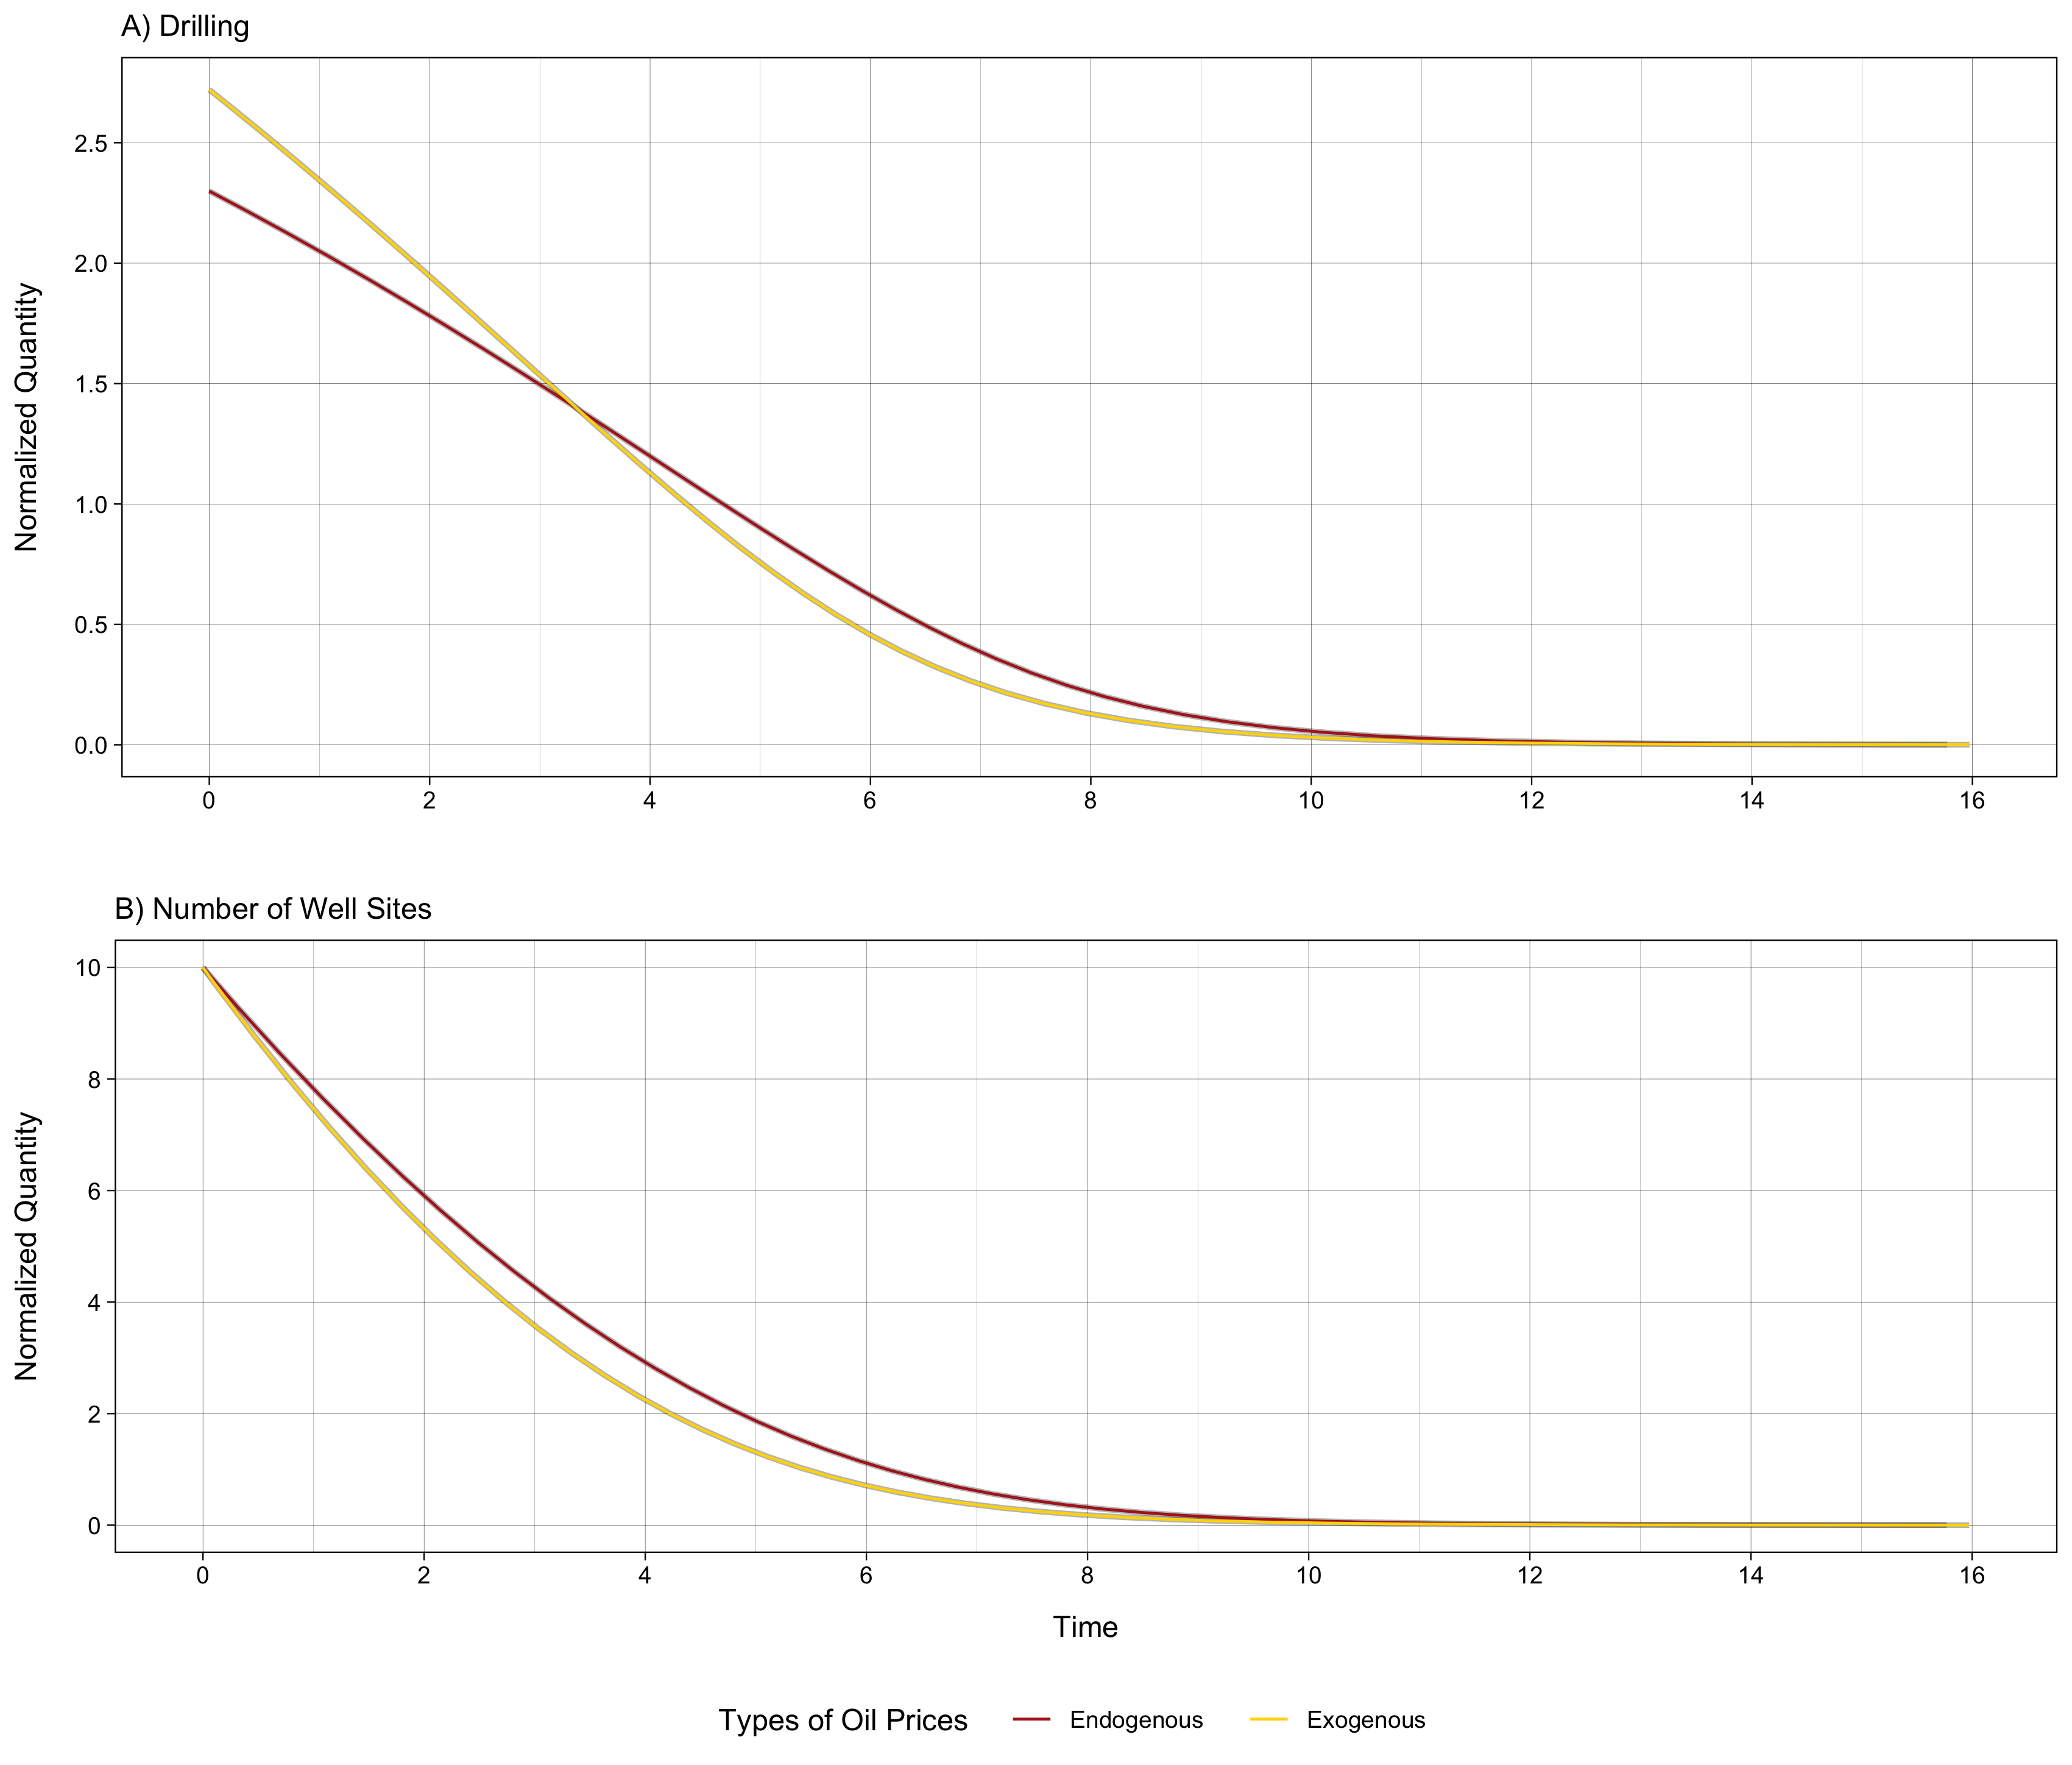
\includegraphics[scale = 0.14]{04_Chapter-3/00A_Figures/Figure_Reserves-and-Drilling-Paths_Endogenous-and-Exogenous-Prices.png}
        \caption{Time Paths for Drilling and Reserves under Endogenous and Exogenous Oil Prices}
        \subcaption*{
            \textit{Note}: 
            This figure depicts differences in the time paths for drilling and reserves under endogenous and exogenous oil prices. This figure takes the assumptions exploited in Figure \ref{Figure:Phase-Diagram_Saddle-Point}, except the initial stock of $R_{0} = 10$ to magnify the differences. See the text for details.
        }
        \label{Figure:Time-Paths-for-Drilling-and-Reserves-under-Endogenous-and-Exogenous-Oil-Prices}
    \end{figure}
}
\clearpage



% Tables
\setcounter{table}{1}
\afterpage{
    \begin{table}
        \centering
        \caption{Summary Statistics for Wells}
        \label{Table:Summary-Statistics-for-Wells}
        \vspace{0.2cm}
        \begin{adjustbox}{scale = 0.85}
            \begin{tabular}{
                >{\raggedright}m{6.0cm}
                >{\raggedleft}m{2.2cm}
                >{\raggedleft}m{2.2cm}
                >{\raggedleft}m{2.2cm}
                >{\raggedleft}m{2.2cm}
                >{\raggedleft\arraybackslash}m{2.2cm}
            }
                \hline \hline
                \multicolumn{1}{c}{} & \multicolumn{1}{c}{Mean} & \multicolumn{1}{c}{(S.D.)} & \multicolumn{1}{c}{P25} & \multicolumn{1}{c}{P50} & \multicolumn{1}{c}{P75} \\
                \hline
                \underline{Production} &  &  &  &  &  \\
                \hspace{0.2cm} Cumulative Oil Production \ (Bbls) & 211,491.30 & (108,012.00) & 136,811.50 & 193,354.00 & 267,052.20 \\
                \hspace{0.2cm} Cumulative Producing Days \ (Days) & 1,451.37 & (356.58) & 1,343.75 & 1,601.00 & 1,697.00 \\
                \underline{Drilling} &  &  &  &  &  \\
                \hspace{0.2cm} Water \ (Bbls) & 101,716.50 & (249,157.50) & 42,032.75 & 65,856 & 130,219.20 \\
                \hspace{0.2cm} Sand/Proppants \ (Lbs) & 4,553,380.00 & (4,560,985.00) & 2,312,951 & 3,441,914 & 5,543,660.00 \\
                \hspace{0.2cm} Horizontal Drilling \ (Feet) & 23,866.77 & (15,134.08) & 19,276.23 & 20,025.88 & 21,227.25 \\
                \underline{Geological Characteristics} &  &  &  &  &  \\
                \hspace{0.2cm} Thickness \ (Feet) & 44.79 & (13.48) & 37.50 & 44.50 & 44.50 \\
                \hspace{0.2cm} Thermal Maturity & 0.64 & (0.20) & 0.50 & 0.50 & 0.75 \\
                \hspace{0.2cm} Total Organic Content & 13.62 & (1.98) & 12.24 & 13.34 & 15.13 \\
                \hline \hline
            \end{tabular}
        \end{adjustbox}
        \begin{minipage}{15.5cm}
            \small \singlespacing
            \textit{Note}: This table presents summary statistics for horizontal wells in our sample.
        \end{minipage}
    \end{table}
}

\clearpage
